\section{Evaluation}

\subsection{Simulation Setup}
We evaluate all receivers with Sionna~\cite{hoydis2022} for $U=2$ UEs and $B=4$ BS antennas, denoted $U\times B\equiv 2\times 4$, in the configuration of \citet{wiesmayr2024}: dual-polarized BS antennas with 3GPP TR 38.901 patterns~\cite{tr38901}, two single-polarized omnidirectional antennas per UE with beamforming $\mathbf{v}=[1,1]^{\mathsf{T}}/\sqrt{2}$, 132 physical resource blocks with 30\,kHz subcarrier spacing at a carrier frequency of 2.14\,GHz, modulation and coding scheme (MCS) index $i=14$ (16-QAM)~\cite[Table~5.1.3.1-1]{ts38214}, and DMRS type A with one additional position.

\begin{figure*}[t]
\centering
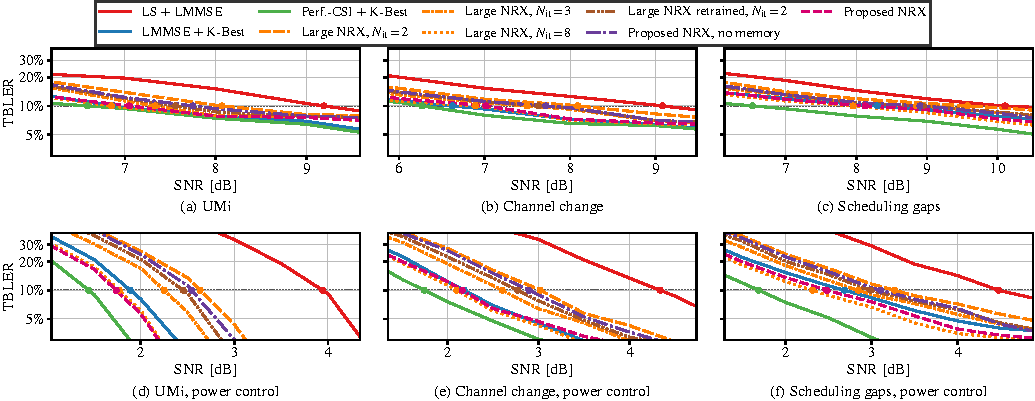
\includegraphics[width=\textwidth]{figures/tbler_vs_snr.pdf}
\caption{TBLER vs.\ SNR for $U\times B\equiv 2\times 4$ MU-MIMO and MCS index $i=14$.}
\label{fig:tbler}
\end{figure*}

To reveal the effect of the memory, we simulate sequences of 64 consecutive slots (32\,ms) over continuously evolving channels. We use 32 sequences for each of the three conditions, all with a new random drop of outdoor UEs per sequence, Doppler shifts up to 400\,Hz, and no path loss or shadow fading:
\begin{itemize}
\item \emph{UMi}: the 3GPP model with the same UE drop for the entire sequence.
\item \emph{Channel change}: UMi, with both UEs switching to a newly drawn channel at slot 33.
\item \emph{Scheduling gaps}: UMi with a pool of four UEs. In every slot, a scheduled UE is replaced with probability 0.25, the DMRS ports are redrawn with probability 0.25, and a UE pauses for up to four slots with a starting probability of 0.05.
\end{itemize}

We compare the proposed NRX with three classical baselines: LS + LMMSE, which uses LS channel estimation with linear interpolation and linear minimum mean square error (LMMSE) detection; LMMSE + K-Best, which uses LMMSE channel estimation and K-Best detection~\cite{guo2006}; and Perf.-CSI + K-Best, which uses K-Best detection with perfect channel state information (CSI).\footnote{Covariance matrices for LMMSE channel estimation are computed per condition from separately simulated channels, and the K-Best detectors apply a list size of $k=64$.} We also compare with the Large NRX of \citet{wiesmayr2024}, pre-trained on UMi channels and evaluated with $N_{\mathrm{it}}\in\{2,3,8\}$, and with the proposed NRX with no memory, which has identical weights but empties the memory before every TB. The LS + LMMSE and K-Best receivers are taken from the code release of \citet{wiesmayr2024}, and the K-Best detectors use one stream when only one UE is scheduled. Both proposed versions use 18 BP iterations, and all other receivers use 20.

We compute the transport block error rate (TBLER) over the TBs in slots 17 to 64, after the memory has filled. All receivers decode identical channels, payloads, and noise realizations. As in the code release, the signal-to-noise ratio (SNR) is rate-adjusted, i.e., $E_b/N_0$.

\subsection{TBLER Performance}
Fig.~\ref{fig:tbler} shows TBLER vs.\ SNR on one evaluation dataset. We call the SNR needed for a TBLER of 10\% the required SNR. The proposed NRX performs close to the Large NRX with $N_{\mathrm{it}}=8$: it is 0.09\,dB behind for UMi, 0.28\,dB ahead for channel change, and 0.10\,dB behind for scheduling gaps. At the same $N_{\mathrm{it}}=2$, the Large NRX requires 1.13\,dB, 1.48\,dB, and 1.53\,dB more, respectively.

The proposed NRX outperforms LS + LMMSE in all three conditions, matches LMMSE + K-Best for UMi and channel change, and is ahead of it for scheduling gaps. Perf.-CSI + K-Best remains ahead of all other receivers.

Unlike the waterfall curves for Double-TDL channels~\cite{wiesmayr2024}, TBLER decreases slowly with SNR for all receivers, including Perf.-CSI + K-Best, because with a fixed beamformer and no power control, some UEs have low channel power.

\subsection{Benefit of the Pilot Memory}
Comparing the proposed NRX with its no-memory version isolates the effect of the memory, as the weights are identical. The memory reduces the required SNR by 0.40\,dB for UMi, 0.34\,dB for channel change, and 0.33\,dB for scheduling gaps.

\begin{figure}[!ht]
\centering
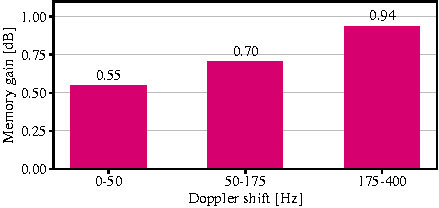
\includegraphics[width=\columnwidth]{figures/memory_gain_vs_doppler.pdf}
\caption{Memory gain in effective SNR at a TBLER of 10\% vs.\ Doppler shift for UMi.}
\label{fig:doppler}
\end{figure}

These gains, however, depend strongly on the channel speed. Fig.~\ref{fig:doppler} shows the memory gain for UMi, grouped by Doppler shift. To remove the effect of low channel power, we evaluate TBLER against the effective SNR, i.e., the SNR plus the effective channel power of the UE in dB. The gain at a TBLER of 10\% is 0.06\,dB for 0--50\,Hz, 0.20\,dB for 50--175\,Hz, and 1.25\,dB for 175--400\,Hz. On slow channels, the proposed NRX with no memory already matches Perf.-CSI + K-Best, leaving little room for improvement by the memory. Each group contains about 10 sequences, so these values are indicative.

We confirm the memory gain on two further independent evaluation datasets at a fixed SNR per condition, chosen for a TBLER near 10\% for the Large NRX on separate data. They also include closely spaced line-of-sight (LOS) UEs, at most $5^\circ$ apart in azimuth, near-far UEs with a received power difference of 6 or 12\,dB, and, on one dataset, channels ray-traced with Sionna RT~\cite{hoydis2023} in the Munich scene of \citet{wiesmayr2024}. The memory lowers TBLER in all of these cases except for closely spaced LOS UEs on one dataset, where it is unchanged, while the Large NRX remains ahead of the proposed NRX in some cases.

\subsection{Latency}
Fig.~\ref{fig:tradeoff} shows the required SNR and median latency for UMi. We time 128 TBs at an SNR of 3\,dB, one TB at a time, in TensorFlow on an NVIDIA A40 GPU. The measurement covers everything after the initial LS estimation and interpolation, including LDPC decoding, CRC, and memory transfers between host and device. These values are not comparable with the real-time budget of 1\,ms in \citet{wiesmayr2024}, which covers neural network inference with TensorRT on an NVIDIA A100 GPU, and our implementation is not real-time capable.

\begin{figure}[!ht]
\centering
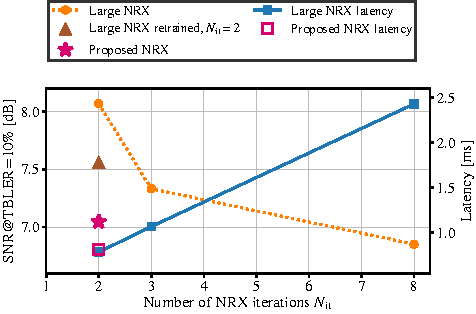
\includegraphics[width=\columnwidth]{figures/snr_latency_tradeoff.pdf}
\caption{SNR performance and median latency vs.\ number of NRX iterations for UMi.}
\label{fig:tradeoff}
\end{figure}

The proposed NRX has a median latency of 41.27\,ms (41.16\,ms with no memory), compared with 40.59\,ms, 43.09\,ms, and 53.05\,ms for the Large NRX with $N_{\mathrm{it}}=2$, 3, and 8, respectively. This is 0.68\,ms more than the Large NRX with $N_{\mathrm{it}}=2$ and 22\% less than with $N_{\mathrm{it}}=8$, at a comparable required SNR.

All results are obtained from simulations with a single training seed.
